\section{Laserové a LED tiskárny}
\label{sec:tiskarny}
Tiskárna je výstupní zařízení, které slouží k přenosu dat uložených v elekronické podobě na papír nebo jiné médium.

Tiskárnu připojujeme k počítači (USB, Bluetooth, Síť\dots), ale může fungovat i samostatně a nebo být přímo součástí multifunčních zařízení jako pokladna nebo lékařské přístroje.
Tiskárny se ovládají pomocí jazyku PCL nebo Postskript.

Kvalitu tisku určuje rozlišení v podobě počtu bodů na palec (DPI) a počtů pixelů na palec (PPI).
Tiskárny nedokáží vytisknout jeden pixel libovolné barvy a tak většinou musí namíchat barvu z několika bodů na jeden pixel obrazu.
Bod proto musí být menší jak pixel.
Výjimku tvoří sublimační tiskárna, která barvy kondenzuje v jednom místě.
\subsection{Laserové tiskárny}
Pracuje na xerografickém principu.
Vyznačují se tichým chodem, nízkými provozními náklady a vysokou rychostí.
Na druhou stanu bývají dražší a potřebují čas na zahřátí.
Není vhodná pro fotografie.
Postup tisku:\\
\begin{enumerate}
  \item Povrch válce se v celé šírce nabije z korony
  \item Válec se osvítí laserem na bodech, které se mají vytisknout, čímž na daném místo sníží odpor polovodiče a náboj se poté z povrchu vybije do středu válce.
  \item Toner, vlivem otáčení nabit stejnou polaritou jako povrch válce, přilne k válci pouze na místech, kde byl odstraněn náboj.
  \item V ostatních místěch je toner od válce odpuzován, protože má stejnou polaritou
  \item Toner se s neutrálním nábojem přenese na papír, který je nabit na opačnou hodnotu než povrch válce
  \item Toner je pomocí teploty $\pm 180\degree C$ a tlaku roztaven a zapečen do papíru
  \item Z papíru je sejmut náboj a papír se uloží do výstupního zásobníku
  \item Mechanický stěrač setře zbytky toneru z válce
  \item Žárovka odstraní náboj z předchozího tisku
\end{enumerate}
\input{TVY-POS/Laserove-a-LED-tiskarny/laser-printer.pdf_tex}
\subsection{LED tiskárny (XEROX)}
Funguje podobně jako laserová tiskárna.
Místo osvícení pomocí laseru se zde využívají dvě a více řad LED diod.
Tudíž se ozařuje celý papír naráz a odpadá nutnost mecahnické části rotace laseru.\\
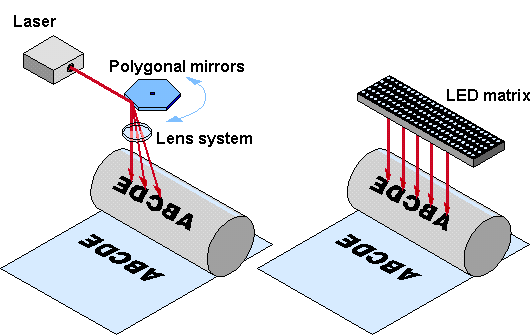
\includegraphics[width=1\linewidth]{TVY-POS/Laserove-a-LED-tiskarny/LEDandLaserPrinter.png}
